\documentclass[preprint,12pt]{elsarticle}

\usepackage{amsmath,amssymb,amsthm,booktabs,graphicx}
\usepackage{microtype}
\usepackage{hyperref}
\hypersetup{hidelinks}
\usepackage{siunitx}
\usepackage{enumitem}
\usepackage{placeins}

\journal{Journal of Computational and Applied Mathematics}

\newtheorem{theorem}{Theorem}
\newtheorem{proposition}[theorem]{Proposition}
\newtheorem{lemma}[theorem]{Lemma}
\newtheorem{corollary}[theorem]{Corollary}
\theoremstyle{remark}
\newtheorem{remark}[theorem]{Remark}

\begin{document}

\begin{frontmatter}

\title{Model-Aware Positive Stieltjes Quadrature:
From Structural Minimax to Gauss--Legendre}

\author[inst1]{Tran Minh Duc\corref{cor1}}
\cortext[cor1]{Corresponding author}
\ead{ductranminh2107@gmail.com}

\affiliation[inst1]{
  organization={FPT University},
  addressline={Lot E2a-7, D1 Street, Saigon Hi-Tech Park},
  city={Ho Chi Minh City},
  country={Vietnam}
}

\begin{abstract}
Generalized Gaussian and rationally exact quadrature already exploit
non-polynomial structure, while rational minimax approximation under
interpolation constraints is an established approximation problem. We
consider the more specific design of positive symmetric
Stieltjes-response quadrature rules that minimize relative error
uniformly over a continuum of Lorentzian widths while matching a
variable prefix of polynomial moments. Within this class, \(n\) positive
node pairs and moment depth \(k\) give the feasible range
\(0\leq k\leq2n\), an admissible dimension \(2n-k\), and the
Gauss--Legendre rule at \(k=2n\). For \(k<2n\), a difference-numerator
degree bound yields a \(2n-k+1\)-point alternation certificate.
High-precision hierarchies for \(n=2,3,4\) quantify the trade-off
between structural accuracy and polynomial protection. For a smooth
residual with Chebyshev coefficients \(|a_j|\leq C\rho^{-j}\), an exact
coefficient-space norm combines with the Lorentzian error to give the
model-aware risk \(G_k(\rho)+\tau S_k\). Conservative numerical
enclosures assign a unique rule on 97.9067\% of the tested parameter
domain. Seventy-two multi-start reconstructions recover the upper-half
rules, and a shifted-Lorentzian stress test supports local rather than
universal robustness. The distinguishing contribution is the combined
positive minimax path, exact selector, and validated decision map, not
positivity, moment matching, or rational approximation separately.
\end{abstract}

\begin{keyword}
numerical quadrature \sep Stieltjes functions \sep rational minimax
approximation \sep moment constraints \sep Gauss--Legendre quadrature
\sep validated numerics
\end{keyword}

\end{frontmatter}

\section{Introduction}

Polynomial exactness is a central organizing principle of numerical
quadrature, but it is not the only way to spend a fixed node budget.
When the dominant difficulty is a nearby pole, quadrature may instead
incorporate rational functions chosen to match that structure
\cite{gautschi1993}. Generalized Gaussian quadrature extends positive
exactness to Chebyshev systems and is naturally described through
moment-space geometry \cite{huybrechs2017}. Positive interpolatory
formulas and optimization-based moment-matching constructions provide
additional general frameworks \cite{vandebos2019,glaubitz2020,
keshavarzzadeh2018}.

A second neighboring direction begins with rational approximation.
Modern algorithms compute rational minimax approximants through adaptive
barycentric representations and Remez-type iterations
\cite{filip2018}. Interpolation-constrained rational minimax
approximation, including higher-order constraints, is also established
\cite{zhang2025}. For Markov and Stieltjes functions, relative rational
approximation has a substantial theory \cite{beckermann2021}. Most
directly, quadrature formulas can be derived from rational
approximations of Cauchy transforms, with poles and residues becoming
nodes and weights and Gauss quadrature connected to Pad\'e approximation
at infinity \cite{horning2025}.

These results rule out several broad novelty claims: pole-aware
quadrature, positive exact quadrature, rational minimax,
equioscillation, and constrained rational approximation are not new
separately. The narrower problem studied here is to combine them in a
model-aware design. At fixed node-pair count, we require a positive
symmetric Stieltjes response, match a variable prefix of polynomial
moments, and minimize relative error uniformly over a continuum of
Lorentzian widths. The resulting family spans a structural minimax rule
and the Gauss--Legendre endpoint. The practical question is then not
only how to compute the rules, but how to select the moment depth when a
smooth uncertain residual is superposed on the structural component.

Within this stated class, the paper makes the following contributions:
\begin{enumerate}[label=(\roman*)]
\item it formulates the positive variable-moment continuum-minimax
problem and characterizes its feasible range, dimension, and
Gauss--Legendre endpoint;
\item it gives a short class-specific degree/zero-count argument leading
to a \(2n-k+1\)-point alternation certificate for every
nonzero-dimensional level;
\item it computes the complete path for \(n=2,3,4\), including the
upper-half levels between the earlier lower-half designs and the
Gaussian endpoint;
\item it derives an exact mixed structural/smooth risk and uses it to
select the moment depth across a two-parameter model domain;
\item it supplies a conservative validated decision map, a shifted-pole
scope test, and independent multi-start reconstruction.
\end{enumerate}

The feasible-range theorem and the Gaussian endpoint are important
structural components of the framework, but are not claimed as
stand-alone inventions of moment or generalized Gaussian theory. A
targeted literature search did not identify a direct source combining
positivity, continuum Lorentzian minimax, variable moment depth, an exact
mixed selector, and a validated parameter partition. This is not an
exhaustive proof of novelty; specialist prior-art review remains
necessary. The claims are restricted to the symmetric positive class
and do not imply universal superiority over Gaussian, adaptive, or
problem-specific quadrature.

\section{Problem formulation}

Let
\[
I[f]=\int_{-1}^{1} f(x)\,dx,
\qquad
L_b(x)=\frac{1}{x^2+b^2},
\qquad
b\in B=[0.08,0.12].
\]
With \(s=b^2\) and \(y=x^2\),
\[
F(s)=I[L_{\sqrt{s}}]
=\int_0^1\frac{y^{-1/2}}{s+y}\,dy
=\frac{2}{\sqrt{s}}\arctan\frac{1}{\sqrt{s}}.
\]
A symmetric \(n\)-pair rule has the form
\[
Q[f]=\sum_{j=1}^{n}w_j\{f(-x_j)+f(x_j)\},
\qquad
0<x_1<\cdots<x_n<1,\quad w_j>0.
\]
Writing \(y_j=x_j^2\), the response on the structural family is the
positive Stieltjes rational function
\[
r_Q(s)=Q[L_{\sqrt{s}}]
=2\sum_{j=1}^{n}\frac{w_j}{s+y_j}.
\]

For an integer \(k\geq0\), define the moment-constrained class
\[
\mathcal A_{n,k}
=
\left\{
Q:
\sum_{j=1}^{n}w_jy_j^\ell=\frac{1}{2\ell+1},
\quad \ell=0,\ldots,k-1
\right\}.
\]
For \(k=0\), no moment condition is imposed.

\begin{lemma}[Equivalent interpretations of the constraints]
For \(k\geq1\), the following conditions are equivalent:
\begin{enumerate}[label=(\alph*)]
\item \(Q\in\mathcal A_{n,k}\);
\item \(Q\) is exact for every polynomial of degree at most \(2k-1\);
\item \(r_Q(s)-F(s)=O(s^{-k-1})\) as \(s\to\infty\).
\end{enumerate}
\end{lemma}

\begin{proof}
Symmetry gives exactness for odd polynomials. For even monomials,
\[
Q[x^{2\ell}]=2\sum_{j=1}^{n}w_jy_j^\ell,
\qquad
I[x^{2\ell}]=\frac{2}{2\ell+1},
\]
which proves the equivalence of (a) and (b). The expansion
\[
\frac{1}{s+y}
=
\sum_{\ell=0}^{m-1}(-1)^\ell y^\ell s^{-\ell-1}
+O(s^{-m-1})
\]
is uniform for \(y\in[0,1]\). Integrating it against
\(y^{-1/2}\,dy\) and applying it to the discrete measure
\(2\sum_jw_j\delta_{y_j}\) proves the equivalence with (c).
\end{proof}

\section{Feasible-range characterization}

Let
\[
\mathcal P_n
=
\{(y,w):
0<y_1<\cdots<y_n<1,\ w_j>0\}
\subset\mathbb R^{2n},
\]
and define the moment map
\[
M_k(y,w)
=
\left(
\sum_{j=1}^{n}w_jy_j^\ell
\right)_{\ell=0}^{k-1}.
\]

\begin{theorem}[Feasible range, dimension, and Gaussian endpoint]
Within the positive ordered class:
\begin{enumerate}[label=(\roman*)]
\item \(\mathcal A_{n,k}\) is nonempty for every \(0\leq k\leq2n\);
\item for \(0\leq k\leq2n\), it is a smooth manifold of dimension
\[
\dim\mathcal A_{n,k}=2n-k;
\]
\item \(\mathcal A_{n,k}\) is empty for \(k>2n\);
\item \(\mathcal A_{n,2n}\) consists of the positive half of the
classical \(2n\)-point Gauss--Legendre rule.
\end{enumerate}
\end{theorem}

\begin{proof}
Nonemptiness follows because the \(2n\)-point Gauss--Legendre rule
satisfies all moment conditions through \(k=2n\), and hence every
prefix.

To prove the rank statement, suppose a linear combination of the rows
of \(DM_k\) vanishes and define
\[
p(y)=\sum_{\ell=0}^{k-1}c_\ell y^\ell.
\]
The columns obtained by differentiating with respect to \(w_j\) give
\(p(y_j)=0\), while the columns obtained by differentiating with respect
to \(y_j\) give \(w_jp'(y_j)=0\). Positivity implies
\(p'(y_j)=0\). Thus every \(y_j\) is a double root. For
\(k\leq2n\), however, \(\deg p\leq2n-1\), so \(p\equiv0\).
Therefore \(DM_k\) has full row rank \(k\), and the implicit-function
theorem gives dimension \(2n-k\).

For impossibility, suppose moments through index \(2n\) were matched.
The polynomial
\[
g(y)=\prod_{j=1}^{n}(y-y_j)^2
\]
has degree \(2n\), is nonnegative, and is not identically zero. The
discrete transformed rule gives \(2\sum_jw_jg(y_j)=0\), whereas
\[
\int_0^1g(y)y^{-1/2}\,dy>0,
\]
a contradiction.

At \(k=2n\), the transformed \(n\)-node rule is exact through degree
\(2n-1\) for the measure \(y^{-1/2}\,dy\). It is therefore its Gaussian
quadrature rule. Under \(y=x^2\), the symmetric rule is exact through
degree \(4n-1\), and hence is the \(2n\)-point Gauss--Legendre rule.
\end{proof}

\begin{remark}
The previously studied range \(0\leq k\leq n\) is the lower half of the
feasible hierarchy. It retains at least \(n\) structural design degrees
of freedom. It is a meaningful high-structural-accuracy regime, but it
is not the maximal feasible range.
\end{remark}

\section{Minimax characterization}

Write two structural responses as \(r_i=p_i/q_i\), where \(q_i\) is
monic of degree \(n\).

\begin{proposition}[Difference-numerator degree]
If \(r_1,r_2\in\mathcal A_{n,k}\) and \(0\leq k\leq2n\), then
\[
r_1-r_2=\frac{H}{q_1q_2},
\qquad
\deg H\leq2n-k-1,
\]
unless the two responses are identical.
\end{proposition}

\begin{proof}
The generic numerator \(p_1q_2-p_2q_1\) has degree at most \(2n-1\).
The shared Laurent coefficients imply
\(r_1-r_2=O(s^{-k-1})\). Since \(q_1q_2\) is monic of degree \(2n\),
the stated degree bound follows.
\end{proof}

Define the relative structural error
\[
\varepsilon_Q(s)=\frac{r_Q(s)}{F(s)}-1.
\]

\begin{theorem}[Alternation certificate]
Let \(0\leq k<2n\). Suppose \(Q^\star\in\mathcal A_{n,k}\) has
\(2n-k+1\) ordered points on the design interval at which
\(\varepsilon_{Q^\star}\) has equal magnitude and alternating sign, and
this magnitude equals its uniform norm. Then no rule in
\(\mathcal A_{n,k}\) has strictly smaller uniform relative error.
\end{theorem}

\begin{proof}
A strictly better competitor would make
\(\varepsilon_{Q^\star}-\varepsilon_Q\) alternate sign at the
\(2n-k+1\) points, forcing at least \(2n-k\) distinct zeros. Since
\(F(s)>0\), these are zeros of \(r_{Q^\star}-r_Q\), contradicting the
degree bound \(2n-k-1\), unless the responses are identical.
\end{proof}

\begin{remark}
The theorem proves minimaxity within the stated class, not global
uniqueness of the nonlinear parameterization. The zero-dimensional
endpoint \(k=2n\) is determined by its moments and does not require a
nontrivial alternation argument.
\end{remark}

\section{Numerical realization of the model-aware path}

The constrained minimax equations combine the \(k\) moment conditions,
equal-magnitude alternating errors, and stationarity at internal
extrema. Lower-half rules were constructed in high precision. The
missing upper-half problems were solved by continuation toward the
Gaussian endpoint and refined through the equioscillation equations.
All published rules have ordered nodes and positive weights.

\begin{table}[ht]
\centering
\caption{Complete \(n=4\) hierarchy. The endpoint \(k=8\) is
zero-dimensional; therefore the alternation-certificate column is not
applicable.}
\label{tab:full-hierarchy}
\small
\begin{tabular}{cccccc}
\toprule
\(k\) & Dimension & Exactness & Cert. points &
Worst relative error & Min. \(w_j\)\\
\midrule
0 & 8 & -- & 9 & 1.490623e-10 & 0.039147 \\
1 & 7 & 1 & 8 & 2.460626e-09 & 0.044528 \\
2 & 6 & 3 & 7 & 4.048641e-08 & 0.051670 \\
3 & 5 & 5 & 6 & 6.653546e-07 & 0.061646 \\
4 & 4 & 7 & 5 & 1.092819e-05 & 0.076595 \\
5 & 3 & 9 & 4 & 1.794333e-04 & 0.101407 \\
6 & 2 & 11 & 3 & 2.943219e-03 & 0.149011 \\
7 & 1 & 13 & 2 & 4.597982e-02 & 0.126194 \\
8 & 0 & 15 & -- & 4.300499e-01 & 0.101229 \\
\bottomrule
\end{tabular}
\end{table}

\begin{figure}[ht]
\centering
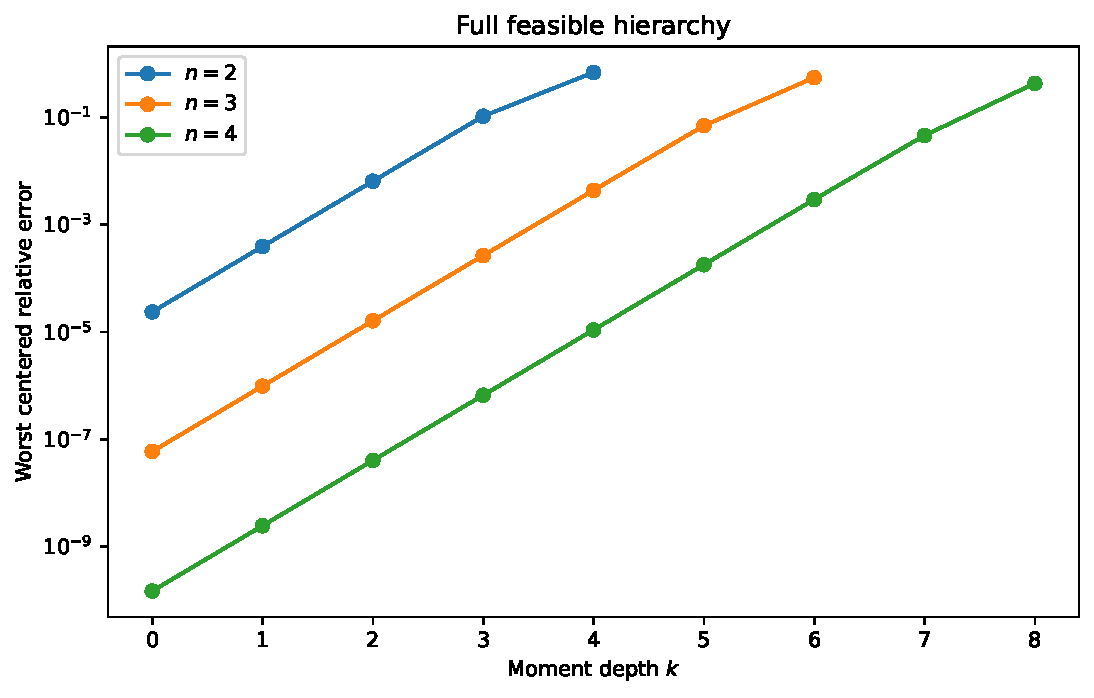
\includegraphics[width=0.84\linewidth]{figures/figure1_full_hierarchy.pdf}
\caption{Worst centered relative error for the full feasible
hierarchies \(0\leq k\leq2n\), \(n=2,3,4\). The final point of each
curve is the corresponding Gauss--Legendre rule.}
\label{fig:full-hierarchy}
\end{figure}

For \(n=4\), the error grows from \(1.49\times10^{-10}\) at \(k=0\) to
\(4.30\times10^{-1}\) at the Gauss endpoint. The upper-half values
\(k=5,6,7\) continue the approximately constant finite-range price per
additional moment before the error enters an order-one regime. This
pattern is empirical and is not claimed as an asymptotic theorem.

\begin{figure}[ht]
\centering
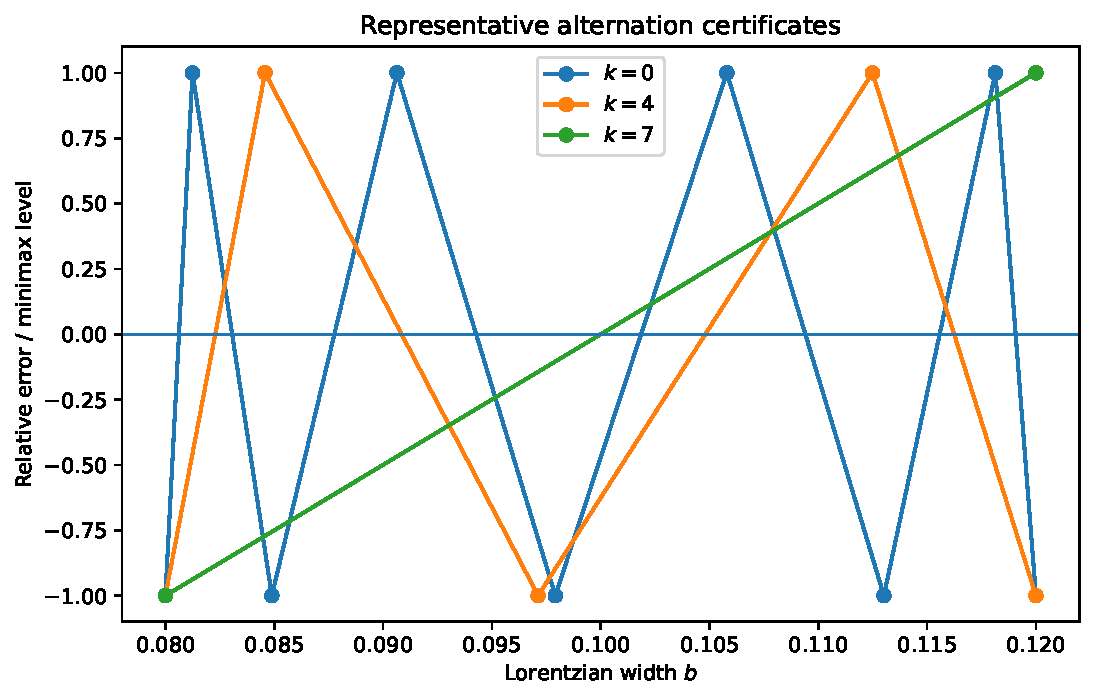
\includegraphics[width=0.82\linewidth]{figures/figure2_alternation.pdf}
\caption{Representative normalized alternation patterns from the lower
endpoint (\(k=0\)), midpoint (\(k=4\)), and upper half (\(k=7\)) of the
\(n=4\) hierarchy.}
\label{fig:alternation}
\end{figure}

\FloatBarrier

\section{Exact coefficient-space rule selection}

Let the uncertain smooth residual have a Chebyshev expansion
\[
h(x)=\sum_{j=0}^{\infty}a_jT_j(x),
\qquad
|a_j|\leq C\rho^{-j},
\quad \rho>1.
\]
For a fixed rule, define
\[
\Delta_j(Q)=I[T_j]-Q[T_j].
\]

\begin{theorem}[Exact coefficient-box norm]
For every fixed bounded quadrature rule,
\[
\sup_h |I[h]-Q[h]|
=
C G_Q(\rho),
\qquad
G_Q(\rho)
=
\sum_{j=0}^{\infty}\rho^{-j}|\Delta_j(Q)|.
\]
\end{theorem}

\begin{proof}
Uniform convergence allows termwise application of \(I-Q\). The
triangle inequality gives the upper bound, and it is attained by the
sign-aligned coefficients
\[
a_j=C\rho^{-j}\operatorname{sign}\Delta_j(Q).
\]
\end{proof}

For the mixed class
\[
f(x)=h(x)+cL_b(x),
\qquad
|c|\leq c_{\max},
\]
define
\[
S_Q=\max_{b\in B}|I[L_b]-Q[L_b]|.
\]

\begin{theorem}[Exact mixed-class risk]
For every fixed rule,
\[
\sup_f |I[f]-Q[f]|
=
C G_Q(\rho)+c_{\max}S_Q.
\]
\end{theorem}

The two signs can be chosen independently. For \(C>0\), define
\(\tau=c_{\max}/C\). The model-aware rule is therefore
\[
k^\star(\rho,\tau)
\in
\arg\min_{0\leq k\leq2n}
\left[G_k(\rho)+\tau S_k\right].
\]

\begin{table}[ht]
\centering
\caption{Full \(n=4\) structural and smooth-risk trade-off at
\(\rho=1.5\).}
\label{tab:risk-components}
\small
\begin{tabular}{ccc}
\toprule
\(k\) & Structural upper enclosure \(S_k\) & \(G_k(1.5)\)\\
\midrule
0 & 5.55627e-09 & 9.11242e-01 \\
1 & 9.17189e-08 & 3.95465e-01 \\
2 & 1.50911e-06 & 2.04657e-01 \\
3 & 2.48007e-05 & 9.59856e-02 \\
4 & 4.07341e-04 & 4.49242e-02 \\
5 & 6.68824e-03 & 2.14018e-02 \\
6 & 1.09706e-01 & 1.17665e-02 \\
7 & 1.71386e+00 & 6.62192e-03 \\
8 & 1.60298e+01 & 3.42291e-03 \\
\bottomrule
\end{tabular}
\end{table}

\begin{figure}[ht]
\centering
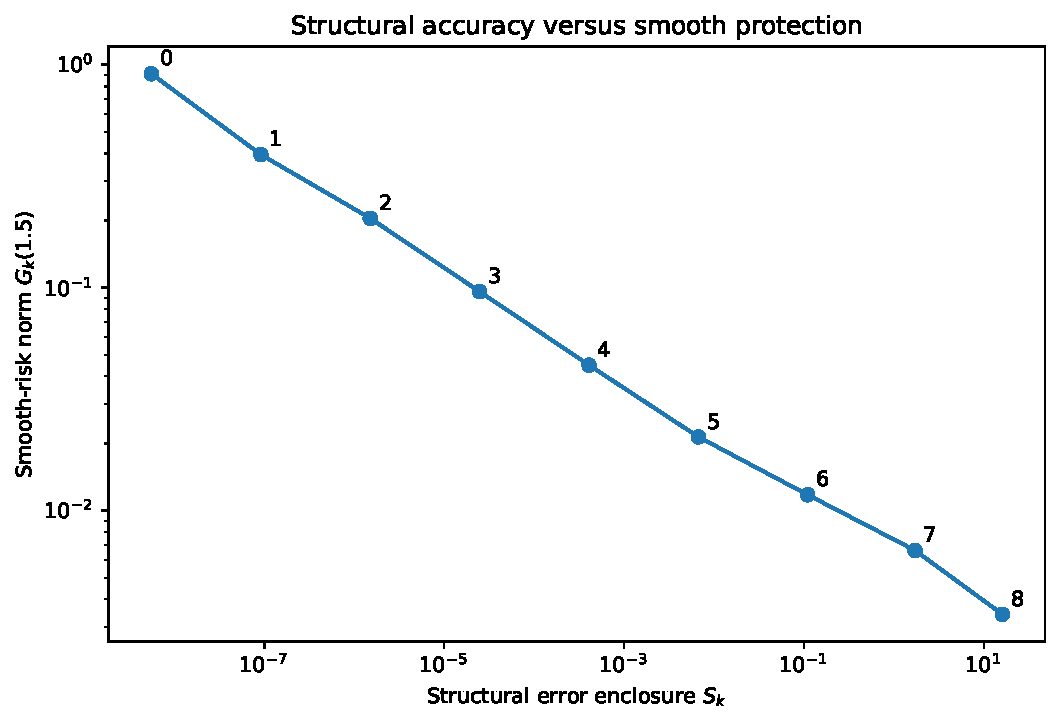
\includegraphics[width=0.78\linewidth]{figures/figure3_risk_tradeoff.pdf}
\caption{Each added moment decreases the smooth-risk norm but increases
the Lorentzian structural error. Labels indicate the moment depth
\(k\).}
\label{fig:risk-tradeoff}
\end{figure}

\section{Validated partition for the rounded rules}

The exact hierarchy theory concerns ideal moment-constrained rules.
Published decimal nodes and weights have small rounding defects.
The coefficient-box risk remains exact for each fixed rounded operator,
but a nominal moment label alone does not transfer exact symbolic
properties.

We therefore re-evaluated all nine rounded \(n=4\) rules. The expected
alternation counts were recovered for \(k=0,\ldots,7\). Structural
errors were enclosed by a dense partition and inflated local derivative
bounds. Chebyshev defects were evaluated through degree 500, and the
remaining tail was bounded geometrically. A parameter cell was assigned
a rule only when its risk upper bound was below the lower bounds of all
competitors throughout the cell.

Adaptive refinement assigned a unique winner on
\[
97.9067\%
\]
of
\[
(\rho,\log_{10}\tau)
\in[1.05,5]\times[-12,12].
\]
The unresolved area, \( 2.0933\% \), is concentrated near
transition curves.

\begin{table}[ht]
\centering
\caption{Fraction of the certified parameter area assigned to each
moment depth.}
\label{tab:selection-fractions}
\small
\begin{tabular}{cc}
\toprule
\(k\) & Certified-area fraction\\
\midrule
0 & 22.279\% \\
1 & 9.216\% \\
2 & 8.299\% \\
3 & 8.463\% \\
4 & 8.478\% \\
5 & 8.460\% \\
6 & 8.117\% \\
7 & 6.934\% \\
8 & 19.753\% \\
\bottomrule
\end{tabular}
\end{table}

\begin{figure}[ht]
\centering
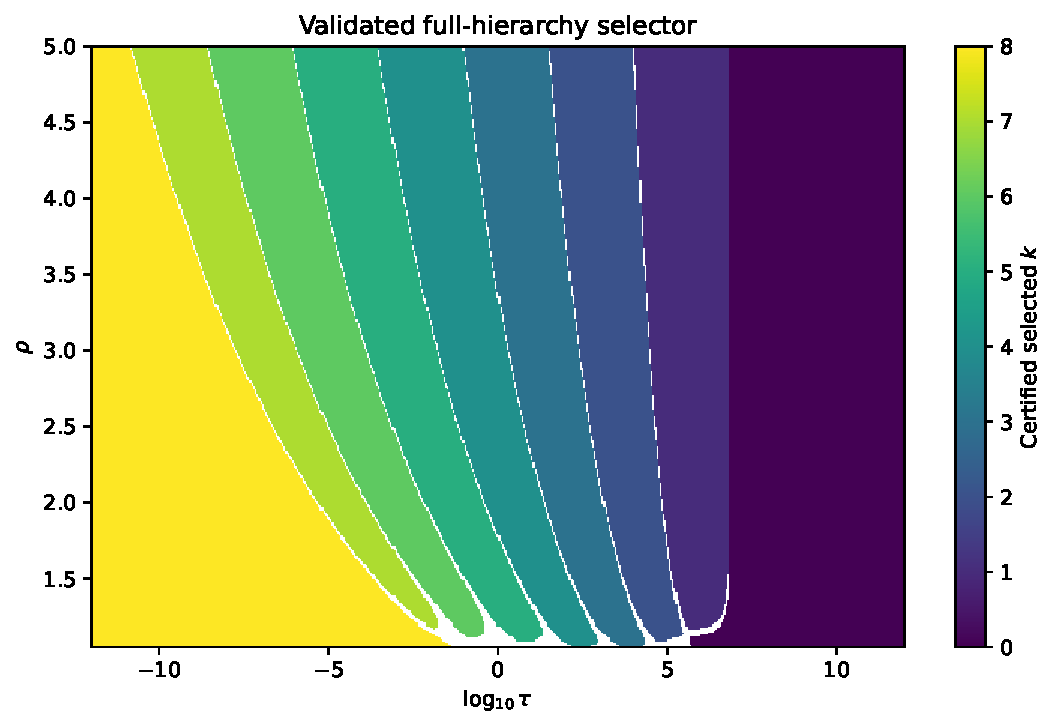
\includegraphics[width=0.84\linewidth]{figures/figure4_certified_selector.pdf}
\caption{Validated full-hierarchy selector. Blank regions are not
assigned because the conservative risk enclosures overlap.}
\label{fig:selector}
\end{figure}

This validation is numerical rather than proof-assistant formal.
The reported coverage depends on the stated enclosures and refinement
depth.

\FloatBarrier

\section{External validity and reconstruction}

\subsection{Small pole-location mismatch}

Without retraining, the centered rules were tested on
\[
L_{a,b}(x)=\frac{1}{(x-a)^2+b^2},
\qquad
|a|\leq0.03,
\quad
0.08\leq b\leq0.12.
\]

\begin{table}[ht]
\centering
\caption{Worst relative errors on the shifted-Lorentzian stress-test
box.}
\label{tab:shifted}
\small
\begin{tabular}{lcccc}
\toprule
Method & Evaluations & Worst error & Worst \(|a|\) & Worst \(b\)\\
\midrule
PMC--k0 & 8 & 4.522336e-06 & 0.0300 & 0.0800 \\
PMC--k4 & 8 & 1.025564e-03 & 0.0300 & 0.0845 \\
Composite--Simpson--9 & 9 & 7.426762e-02 & 0.0300 & 0.1200 \\
Gauss--Legendre--8 & 8 & 4.300499e-01 & 0.0000 & 0.0800 \\
\bottomrule
\end{tabular}
\end{table}

\begin{figure}[ht]
\centering
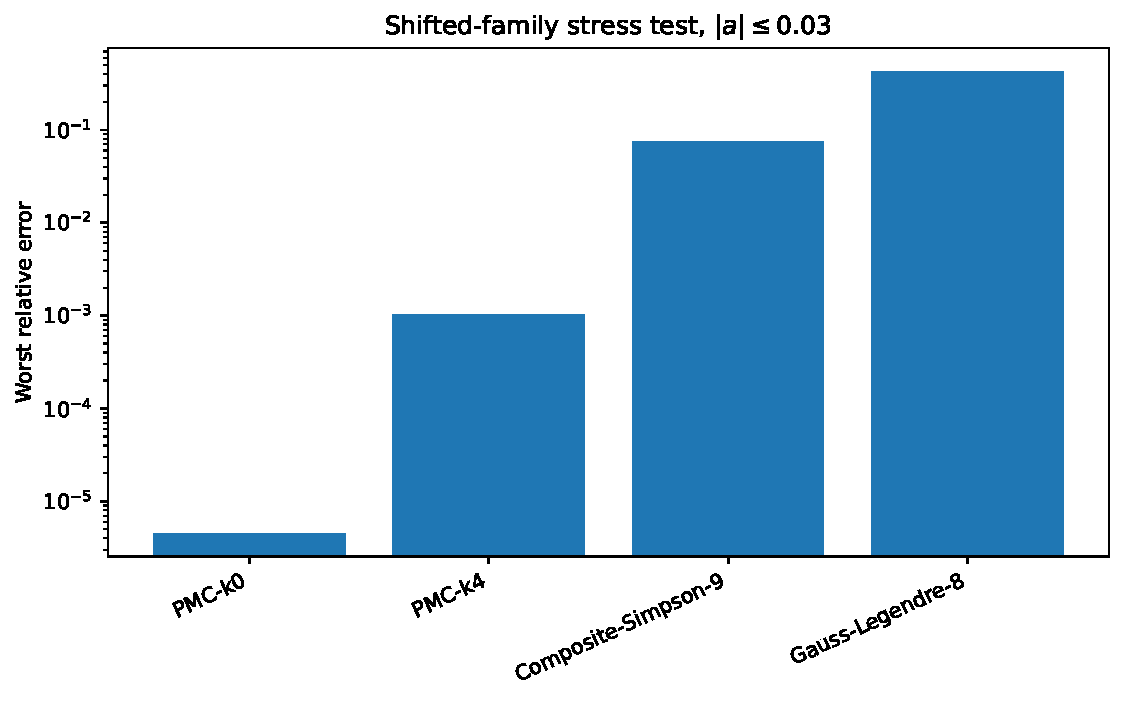
\includegraphics[width=0.82\linewidth]{figures/figure5_shifted_stress.pdf}
\caption{Stress test under small pole-location mismatch. The comparison
supports local structural robustness, not shifted-family minimaxity or
universal superiority.}
\label{fig:shifted}
\end{figure}

The \(k=0\) rule has worst relative error
\(4.52\times10^{-6}\), whereas the Gauss endpoint has worst error
\(4.30\times10^{-1}\) on the same box. The centered error is nevertheless
inflated by more than four orders of magnitude, so the correct
interpretation is local robustness rather than shift invariance.

\subsection{Independent multi-start reconstruction}

The six upper-half problems
\[
(2,3),\ (3,4),\ (3,5),\ (4,5),\ (4,6),\ (4,7)
\]
were reconstructed from twelve perturbed starts each. A run was accepted
only when nodes were ordered, weights were positive, moment residuals
were below \(10^{-10}\), and scaled equioscillation residuals were below
\(10^{-8}\).

\begin{table}[ht]
\centering
\caption{Independent multi-start reconstruction of the upper-half
rules. Error differences are relative to the published minimax level.}
\label{tab:multistart}
\scriptsize
\begin{tabular}{ccccc}
\toprule
\((n,k)\) & Accepted starts & Error difference &
Max. node difference & Max. weight difference\\
\midrule
$(2,3)$ & 12/12 & 2.64e-16 & 5.55e-17 & 5.55e-17 \\
$(3,4)$ & 10/12 & 6.78e-14 & 4.44e-16 & 5.00e-16 \\
$(3,5)$ & 12/12 & 5.31e-14 & 1.29e-14 & 1.32e-14 \\
$(4,5)$ & 8/12 & 2.38e-12 & 4.44e-15 & 4.27e-15 \\
$(4,6)$ & 11/12 & 9.22e-14 & 1.03e-14 & 1.05e-14 \\
$(4,7)$ & 12/12 & 5.11e-13 & 8.95e-14 & 6.43e-14 \\
\bottomrule
\end{tabular}
\end{table}

All accepted solutions in each problem formed a single error-level
cluster. No accepted start found a better rule by more than
\(10^{-6}\) relative, and the maximum best-rule error difference was
\(2.38\times10^{-12}\). This reduces the risk of a local numerical
artifact but is not a proof of global uniqueness or third-party
replication.

\section{Relation to prior work and novelty scope}

\subsection{Structure-aware and generalized quadrature}

Gautschi's rational Gauss-type rules establish the principle that a
quadrature formula can integrate rational functions selected to match
important external poles \cite{gautschi1993}. The present work therefore
does not introduce pole-aware quadrature. Its structural objective is
different: it minimizes relative error over a continuum of Lorentzian
widths instead of enforcing exactness at a finite set of prescribed
poles.

Generalized Gaussian quadrature for Chebyshev systems supplies positive
interior-node rules exact for non-polynomial spaces, and complete
Chebyshev systems support stepwise increases in exactness
\cite{huybrechs2017}. Positive exact formulas and positive-node
geometry are also well developed \cite{vandebos2019,glaubitz2020}.
Accordingly, neither positivity nor an ordered hierarchy of exactness is
claimed as new. Here the moment depth indexes a family selected by a
continuum Stieltjes minimax criterion at fixed node-pair count.

Optimization-based nested quadrature shows that nonlinear
moment-matching systems can be solved flexibly
\cite{keshavarzzadeh2018}. Our nonlinear solver and multi-start study
are reproducibility mechanisms, not the principal conceptual
contribution.

\subsection{Rational approximation and minimax constraints}

Rational minimax approximation and equioscillation are classical;
adaptive barycentric algorithms make high-order problems computationally
accessible \cite{filip2018}. Interpolation-constrained rational minimax
approximation already includes prescribed function values and
higher-order derivative conditions \cite{zhang2025}. After the change
of variable \(z=1/s\), matching Laurent coefficients at infinity is
closely related to confluent interpolation at \(z=0\). Thus the novelty
claim cannot be ``minimax plus constraints.'' The alternation theorem in
this paper is instead a concise specialization to positive
Stieltjes-response quadrature, where the shared coefficients reduce the
difference-numerator degree.

Markov-function rational approximation provides especially relevant
relative-error context \cite{beckermann2021}. Horning and Trefethen make
the approximation-to-quadrature bridge explicit by deriving quadrature
from rational approximations of Cauchy transforms; their framework also
connects Gauss quadrature with Pad\'e approximation at infinity
\cite{horning2025}. This is the closest conceptual comparator. The
distinction here is the simultaneous enforcement of positive residues,
a variable polynomial-moment prefix, a continuum relative-minimax
objective, and an exact mixed-class selector.

\subsection{Worst-case rule selection}

Worst-case analysis for analytic function classes is an established
part of quadrature theory \cite{trefethen2022,goda2024}, and recent
positive-weight kernel quadrature gives a different
convex-geometric worst-case framework \cite{hayakawa2026}. The
coefficient-box identity used here is elementary duality. Its role is
to make the smooth residual commensurate with the Stieltjes structural
error, producing
\[
G_k(\rho)+\tau S_k.
\]
The paper's practically distinctive output is therefore not a new norm
identity in isolation, but a selector and validated decision map over a
finite family of positive structural rules.

\subsection{Defensible novelty statement}

The targeted audit found no direct source combining all of the
following: positive symmetric Stieltjes residues, continuum Lorentzian
relative minimax, variable moment depth at fixed node-pair count, an
exact mixed smooth/structural selector, and a validated parameter
partition. The defensible claim is this combined model-aware framework.
The paper does not claim to invent positivity, moment matching,
structure-aware quadrature, constrained rational minimax,
equioscillation, or the Gauss/Pad\'e connection separately.

\section{Limitations}

The theoretical and numerical study is one-dimensional and symmetric.
The principal structural family is the centered Lorentzian kernel.
The shifted-family experiment is a stress test and is not itself
minimax-optimized or formally interval-certified. Global uniqueness of
the nonlinear minimax parameters is not proved. The full selector
validation leaves approximately 2.0933\% of the domain unassigned. The
empirical near-geometric price per moment is not an asymptotic theorem.

The literature audit is targeted rather than exhaustive. Equivalent
constructions may exist under the language of moment spaces,
generalized Gaussian quadrature, constrained Markov approximation, or
interpolatory rational minimax. For this reason, the manuscript avoids
``first'' and ``unprecedented'' claims and retains specialist novelty
review as a submission requirement. The phrase ``validated numerical
partition'' refers to conservative computational enclosures, not
proof-assistant verification.

\section{Conclusion}

Within the stated positive symmetric Stieltjes class, the variable
moment depth organizes a path
\[
k=0
\quad\longrightarrow\quad
k=2n
\]
from a structural minimax rule to Gauss--Legendre. The
feasible-range characterization and difference-degree argument support
the numerical construction, while the exact mixed risk turns the family
into a model-aware selector. Complete computations for \(n=2,3,4\),
conservative decision-map validation, a shifted-pole stress test, and
multi-start reconstruction quantify both the promise and the limits of
the approach.

The main contribution is not any ingredient separately. It is the
combination of positive Stieltjes realization, continuum structural
minimax, variable polynomial protection, and exact rule selection in one
computable framework. The next scientific step is independent
specialist comparison with the closest generalized-quadrature and
constrained-rational literature, followed by extensions beyond symmetry
and the centered kernel.

\section*{Data and code availability}

The code, published rules, generated data, and reproduction scripts are
available at
\url{https://github.com/TurkeyOp/partial-moment-stieltjes-quadrature}.
The Version 2 upper-half and full-selector materials are included in the
accompanying research archive and should be merged into the public
repository before journal submission.

\section*{Funding}

This research did not receive any specific grant from funding agencies
in the public, commercial, or not-for-profit sectors.

\section*{Declaration of competing interest}

The author declares that he has no known competing financial interests
or personal relationships that could have appeared to influence the
work reported in this paper.

\section*{Declaration of generative AI and AI-assisted technologies in
the manuscript preparation process}

During the preparation of this work, the author used OpenAI ChatGPT to
assist with literature organization, code prototyping, manuscript
structuring, and language revision. The author reviewed and verified
the mathematical derivations, numerical results, references,
interpretations, and final wording and takes full responsibility for
the content of the article.

\begin{thebibliography}{13}
\providecommand{\url}[1]{\texttt{#1}}

\bibitem{gautschi1993}
W. Gautschi, Gauss-type quadrature rules for rational functions,
arXiv:math/9307223 (1993).

\bibitem{huybrechs2017}
D. Huybrechs, On the computation of Gaussian quadrature rules for
Chebyshev sets of linearly independent functions,
arXiv:1710.11244 (2017).

\bibitem{filip2018}
S.-I. Filip, Y. Nakatsukasa, L. N. Trefethen, B. Beckermann,
Rational minimax approximation via adaptive barycentric
representations, arXiv:1705.10132 (2017).

\bibitem{zhang2025}
L.-H. Zhang, Y.-N. Zhang, b-d-Lawson: a method for the interpolation
constrained rational minimax approximation,
arXiv:2502.10665 (2025).

\bibitem{horning2025}
A. Horning, L. N. Trefethen, Quadrature formulas from rational
approximations, arXiv:2507.14971 (2025).

\bibitem{vandebos2019}
L. M. M. van den Bos, B. Sanderse, A geometric approach for the
addition of nodes to an interpolatory quadrature rule with positive
weights, arXiv:1902.07477 (2019).

\bibitem{glaubitz2020}
J. Glaubitz, Constructing positive interpolatory cubature formulas,
arXiv:2009.11981 (2020).

\bibitem{keshavarzzadeh2018}
V. Keshavarzzadeh, R. M. Kirby, A. Narayan, Generation of nested
quadrature rules for generic weight functions via numerical
optimization: Application to sparse grids, arXiv:1808.03707 (2018).

\bibitem{beckermann2021}
B. Beckermann, J. Bisch, R. Luce, On the rational approximation of
Markov functions, with applications to the computation of Markov
functions of Toeplitz matrices, arXiv:2106.05098 (2021).

\bibitem{trefethen2022}
L. N. Trefethen, Exactness of quadrature formulas,
arXiv:2101.09501 (2021).

\bibitem{goda2024}
T. Goda, Y. Kazashi, K. Tanaka, How sharp are error bounds? Lower
bounds on quadrature worst-case errors for analytic functions,
arXiv:2401.07196 (2024).

\bibitem{hayakawa2026}
S. Hayakawa, Convex-geometric error bounds for positive-weight kernel
quadrature, arXiv:2605.05705 (2026).

\bibitem{nailwal2024}
R. Nailwal, A. Zalar, Gaussian quadratures with prescribed nodes via
moment theory, arXiv:2412.20849 (2024).

\end{thebibliography}

\end{document}
